\documentclass[a4paper,twocolumn]{article}
\usepackage[colorlinks=true]{hyperref}
\usepackage{graphicx}
% From libnqsbtls.tex
\usepackage{xcolor,listings}

\newcommand\inputml[1]{\lstinputlisting[language={[Objective]Caml}]{#1}}

\lstdefinelanguage{OCaml}{
  keywords={
    and,as,assert,asr,begin,class,constraint,do,done,downto,effect,else,end,exception,
    external,false,for,fun,function,functor,if,implicit,in,include,inherit,initializer,
    land,lazy,let,lor,lsl,lsr,lxor,macro,match,method,mod,module,mutable,new,object,
    of,open,or,private,rec,sig,struct,then,to,true,try,type,val,virtual,when,
    with,while},
  comment=[s]{(*\ }{\ *)},
}

\definecolor{darkgreen}{rgb}{0,0.2,0}
\definecolor{darkblue}{rgb}{0.1,0.1,0.8}
\definecolor{darkbrown}{rgb}{0.5,0.3,0.0}
\definecolor{grey}{rgb}{0.5,0.5,0.5}
\definecolor{darkgrey}{rgb}{0.2,0.2,0.2}

\lstdefinestyle{ocaml}{
  basicstyle=\ttfamily, % \small
  basewidth=0.5em,
  commentstyle=\color{darkgreen},
  escapeinside={(**}{)},
  keywordstyle=\color{darkblue},
  language=OCaml,
  morekeywords={macro},
  stringstyle=\color{blue},
  showstringspaces=false,
  mathescape=true,
  moredelim=**[is][]{?}{?},
  moredelim=**[is][]{&}{&},
}

\lstset{literate=%
{->}{{$\to$}}2
{...}{{$\ldots$}}2
}

\begin{document}

\title{Experiences with Effects}
\author{Thomas Leonard\and
        Craig Ferguson\and
        Patrick Ferris\and
        Sadiq Jaffer\and
        Tom Kelly\and
        KC Sivaramakrishnan\and
        Anil Madhavapeddy}
\maketitle

\begin{abstract}
The multicore branch of OCaml adds support for \emph{effect handlers}.
In this talk, we report our experiences with effects,
both from converting existing code, and from writing new code.
Converting the Angstrom parser from a callback style to effects
greatly simplified the code, while also improving performance and reducing allocations.
Our experimental Eio library uses effects to allow writing concurrent code in direct style,
without the need for monads (as found in Lwt or Async).

\end{abstract}

\section*{Effects}

The multicore branch of OCaml adds support for \emph{effect handlers}\footnote{Retrofitting Effect Handlers onto OCaml, accepted to PLDI 2021}.
Using effects brings several advantages over using callbacks or monadic style:

\begin{itemize}
\item It is faster, because no heap allocations are needed to simulate a stack.
\item Concurrent code can be written in the same style as plain non-concurrent code.
\item Because a real stack is used, exception backtraces and stack-based profiling work as expected.
\item Other features of the language (such as {\tt try}/{\tt with}, {\tt match}, {\tt while}, etc)
can be used in concurrent code.
\end{itemize}

Installing an effect handler executes a function in a new stack, called a \emph{fibre}.
The function can \emph{perform} an effect (similar to raising an exception), transferring control to the handler.
Unlike an exception handler, an effect handler also receives a \emph{continuation},
which can be used to resume the suspended fibre when the handler is ready.

\section*{Angstrom with effects}

A natural implementation for a parser is a function that takes an input stream and returns the parsed result.
This works well if the complete input is present at the start, or if the application can block while waiting for more data.

However, if the parser needs to run concurrently with other code (as is typical in a network service), then this API needs to change so that when it requires more input the parser returns a callback to the application.
Angstrom\footnote{\url{https://github.com/inhabitedtype/angstrom/}} is a parser-combinator library written in this way.
It is intended for high-performance applications, such as network protocols.

To give a quick idea of the difference between the callback style and the direct style, here is Angstrom's implementation of the \verb|*>| combinator (which uses a pair of parsers \verb|a| and \verb|b| to parse a pair of items, discarding the first result):
\begin{lstlisting}[style=ocaml]
let (*>) a b =
  { run = fun input pos more fail succ ->
    let succ' input' pos' more' _ =
      b.run input' pos' more' fail succ in
    a.run input pos more fail succ'
  }
\end{lstlisting}

Here is the same thing written in direct style (without support for asynchronous reads):
\begin{lstlisting}[style=ocaml]
let (*>) a b state =
  let _ = a state in
  b state
\end{lstlisting}

% Mention use of exceptions?

But now, thanks to effects, the simpler direct-style version \emph{does} support asynchronous reads.
If the \verb|a| or \verb|b| parser needs more input, it can perform an effect to get it.

Interestingly, our ``effects" version of Angstrom doesn't actually perform or handle any effects.
Instead, it allows the user to provide a function for reading more data;
if that function happens to perform an effect that suspends the parsing operation during the read
then other threads will be able to run while the parser is waiting for the read to complete.

An initial benchmark (parsing an HTTP request) shows that the simpler direct-style version of Angstrom is also slightly faster, and performs considerably fewer allocations:

\begin{figure}[h]
\begin{tabular}{l|rrrrr}
          & Time     & MinWrds &  MajWrds \\
\hline
Callbacks & 11.18ms  & 4640k   &    50471 \\
Effects   & 10.46ms  & 1066k   &      285 \\
\end{tabular}
\end{figure}

We can also implement the old (callback-based) API on top of the new one, for compatibility.
The refill-buffer effect is only performed rarely, and so we only allocate a callback occasionally,
when more data is actually needed, not for every parsing operation.


\section*{Effects-based IO}

It is easy to use effects to implement a cooperative scheduler,
by running each thread in its own fibre.
Threads perform effects when they want to block (e.g. for IO).
The scheduler handles the effect by saving the continuation in the IO operation and resuming the next runnable thread.

Our experimental new IO library\footnote{\url{https://github.com/ocaml-multicore/eio}}
does this to provide direct-style IO, without the need for monads.
The library aims to support multiple platforms using optimised platform-specific backends,
such as {\tt io\_uring}\footnote{\url{https://kernel.dk/io_uring.pdf}} on Linux and
Grand Central Dispatch\footnote{\url{https://developer.apple.com/documentation/DISPATCH}} on macos.

In the talk we will demonstrate the current state of the library, and provide comparisons between Lwt and Eio.

\section*{HTTP benchmarks}

Results from our preliminary benchmarking of HTTP servers indicate that an effect-based IO library is competitive both with callback-based OCaml implementatons but also commonly used frameworks in other languages, such as Go's \emph{net/http}. There remains a performance gap between the OCaml implementations and high performing Rust ones, the closing of which is a goal we intend to provide more progress on in the talk.

\begin{figure}[hbtp]
\caption{HTTP throughput comparison}
\centering
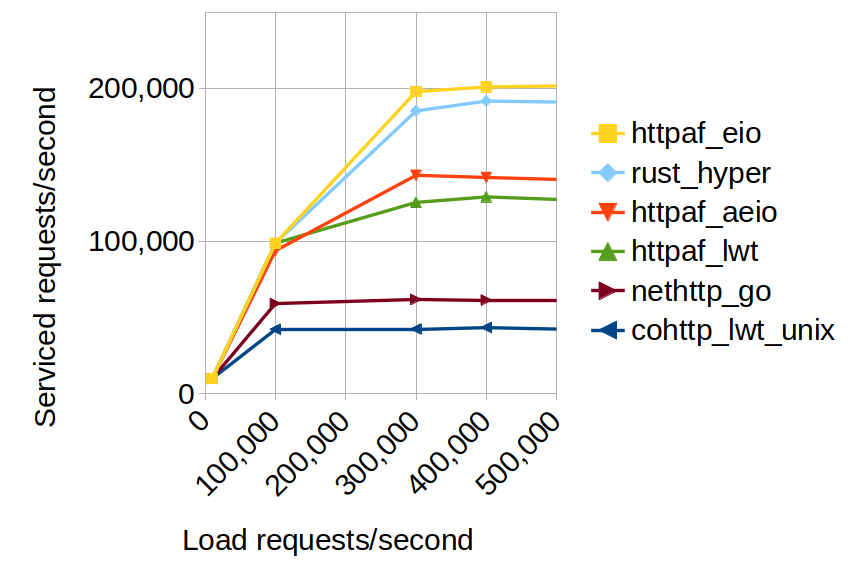
\includegraphics[width=0.45\textwidth]{rps-graph.png}
\end{figure}

Figure 1 shows a throughput comparison of several HTTP server implementations:
\begin{itemize}
\item OCaml 4.12 with cohttp 4.0 and Lwt 5.4.0 (cohttp\_lwt\_unix)
\item OCaml 4.12 with httpaf 0.7.1 and Lwt 5.4.0 (httpaf\_lwt)
\item OCaml 4.12+domains+effects with 0.7.1 and aeio 0.2.0 (httpaf\_effects)
\item Go 1.15.4 with net/http (nethttp\_go)
\item rust 1.47.0 with hyper 0.12 and tokio 0.1.11 (rust\_hyper)
\end{itemize}

All benchmarks were restricted to one core. The results above were from an Intel(R) Xeon(R) Silver 4108 CPU with turbo disabled running Ubuntu 18.04.3 LTS and Linux 4.15.0-65-generic. Code for the specific run used for benchmarking can be found at https://github.com/ocaml-multicore/retro-httpaf-bench/tree/ocamlworkshop2021 .

\end{document}
